% Neural network diagram
% Made with Xematics. Positions are in px (1 px = 0.75 pt), as in the SVG export.
\documentclass[tikz, border=4pt]{standalone}
\definecolor{xm1}{HTML}{15191F}
\definecolor{xm2}{HTML}{9AA3AE}
\definecolor{xm3}{HTML}{56B4E9}
\definecolor{xm4}{HTML}{9FD4F3}
\definecolor{xm5}{HTML}{2B313B}
\definecolor{xm6}{HTML}{E8EAED}
\definecolor{xm7}{HTML}{1C2128}
\definecolor{xm8}{HTML}{6B7480}
\definecolor{xm9}{HTML}{24506B}
\definecolor{xm10}{HTML}{7CC4EE}
\definecolor{xm11}{HTML}{4F4B22}
\definecolor{xm12}{HTML}{E6DC6A}
\definecolor{xm13}{HTML}{E69F00}
\definecolor{xm14}{HTML}{F3C45C}
\begin{document}
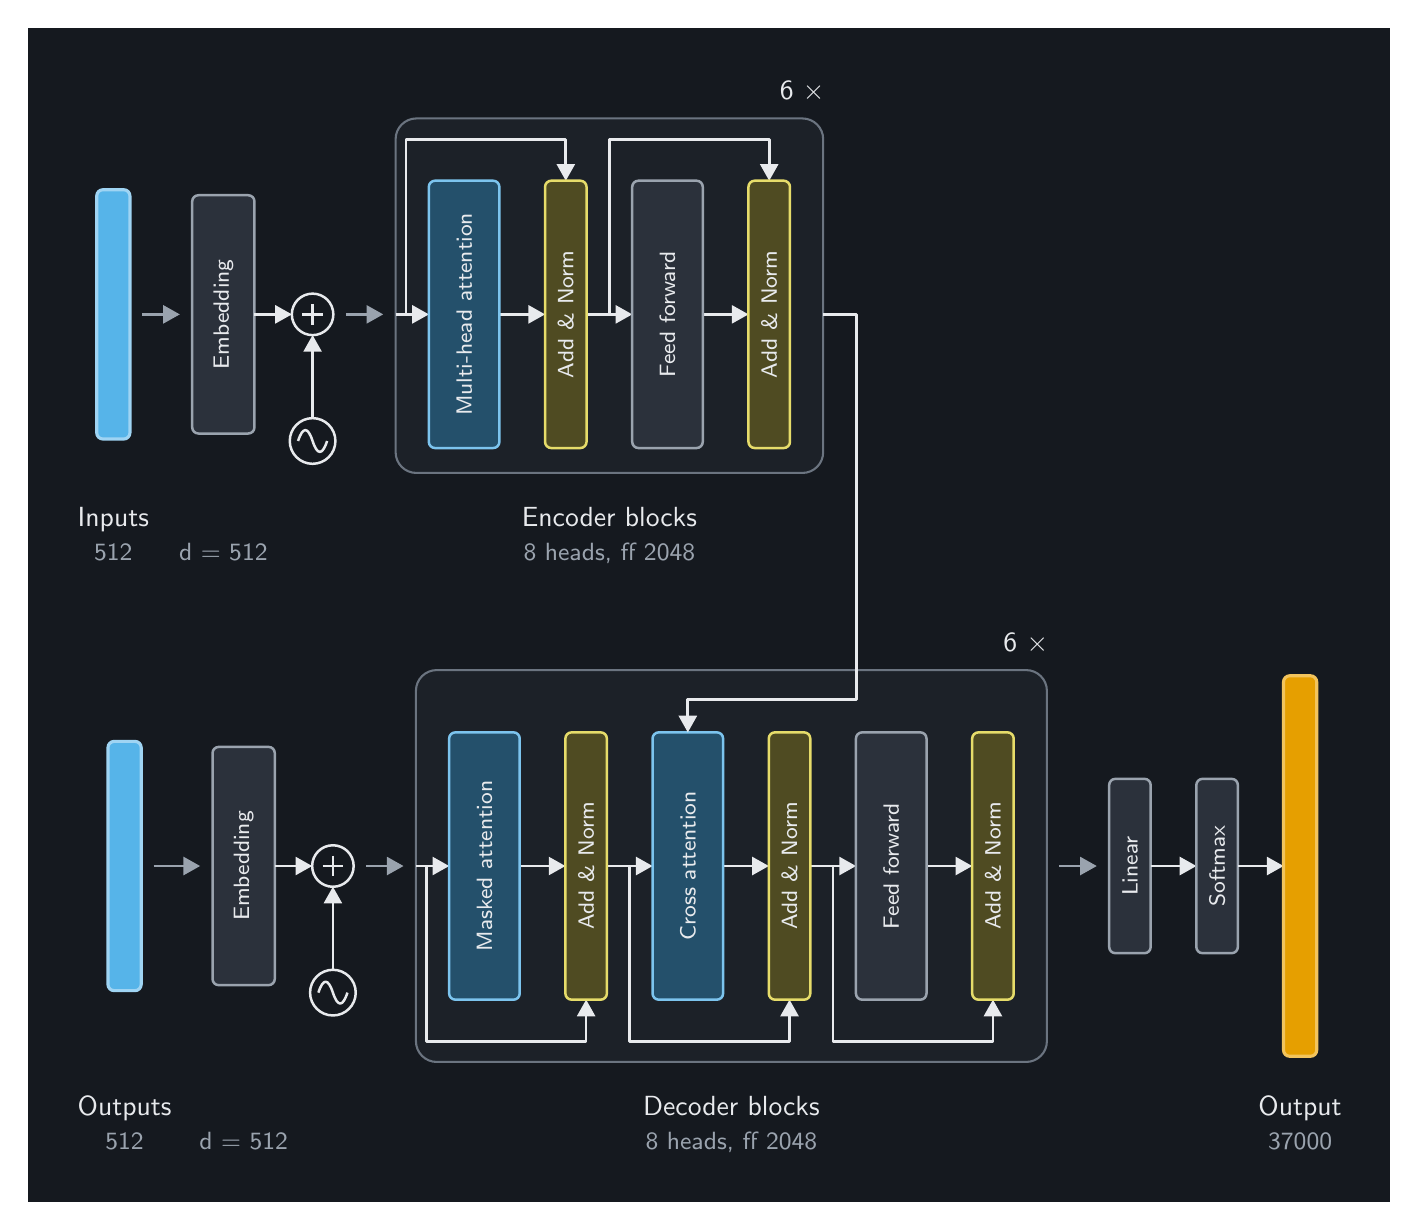
\begin{tikzpicture}[x=0.75pt, y=-0.75pt]
  \tikzset{
    xm arrow d6rgep/.style={draw=xm2, line width=1.05pt},
    xm arrow 14mtdps/.style={fill=xm2, line join=round},
    xm box 1j16zct/.style={fill=xm3, draw=xm4, line width=1.13pt, rounded corners=2.25pt},
    xm box sz2eev/.style={fill=xm5, draw=xm2, line width=0.9pt, rounded corners=2.25pt},
    xm text xm6/.style={text=xm6, inner sep=0},
    xm flow 1kpdjph/.style={draw=xm6, line width=0.95pt},
    xm flow 19pejvw/.style={fill=xm6, line join=round},
    xm op ezqd0u/.style={fill=xm1, draw=xm6, line width=0.9pt},
    xm op 1461dhn/.style={draw=xm6, line width=0.98pt, line join=round},
    xm op 1rsfh3v/.style={draw=xm6, line width=0.9pt, line join=round},
    xm frame z69o9f/.style={fill=xm7, draw=xm8, line width=0.75pt, rounded corners=7.5pt},
    xm residual 1og8xv2/.style={draw=xm6, line width=0.95pt, line join=round},
    xm residual 19pejvw/.style={fill=xm6, line join=round},
    xm box mghmh4/.style={fill=xm9, draw=xm10, line width=0.9pt, rounded corners=2.25pt},
    xm box 1azwj0l/.style={fill=xm11, draw=xm12, line width=0.9pt, rounded corners=2.25pt},
    xm box bwc7cf/.style={fill=xm13, draw=xm14, line width=1.13pt, rounded corners=2.25pt},
    xm memory 1dkuply/.style={draw=xm6, line width=1.05pt, line join=round},
    xm memory 19pejvw/.style={fill=xm6, line join=round},
    xm text xm2/.style={text=xm2, inner sep=0},
  }
  \fill[xm1] (0,0) rectangle (656.3,565.55);
  % Diagram
  \path[xm arrow d6rgep] (55.27,138.13) -- (66.27,138.13);
  \path[xm arrow 14mtdps] (73.27,138.13) -- (65.27,142.63) -- (65.27,133.63) -- cycle;
  \path[xm arrow d6rgep] (153.27,138.13) -- (164.27,138.13);
  \path[xm arrow 14mtdps] (171.27,138.13) -- (163.27,142.63) -- (163.27,133.63) -- cycle;
  \path[xm arrow d6rgep] (60.69,403.91) -- (76.06,403.91);
  \path[xm arrow 14mtdps] (83.06,403.91) -- (75.06,408.41) -- (75.06,399.41) -- cycle;
  \path[xm arrow d6rgep] (163.06,403.91) -- (174.06,403.91);
  \path[xm arrow 14mtdps] (181.06,403.91) -- (173.06,408.41) -- (173.06,399.41) -- cycle;
  \path[xm arrow d6rgep] (497.06,403.91) -- (508.06,403.91);
  \path[xm arrow 14mtdps] (515.06,403.91) -- (507.06,408.41) -- (507.06,399.41) -- cycle;
  \path[xm box 1j16zct] (33.27,78.07) rectangle ++(16,120.12);
  \path[xm box sz2eev] (79.27,80.73) rectangle ++(30,114.8);
  \node[xm text xm6, font=\sffamily\fontsize{8.25}{9.9}\selectfont, anchor=center, rotate=90] at (94.27,138.13) {Embedding};
  \path[xm flow 1kpdjph] (109.27,138.13) -- (120.27,138.13);
  \path[xm flow 19pejvw] (127.27,138.13) -- (119.27,142.63) -- (119.27,133.63) -- cycle;
  \path[xm op ezqd0u] (137.27,138.13) circle[radius=10];
  \path[xm op 1461dhn] (132.27,138.13) -- (142.27,138.13) (137.27,133.13) -- (137.27,143.13);
  \path[xm flow 1kpdjph] (137.27,188.13) -- (137.27,155.13);
  \path[xm flow 19pejvw] (137.27,148.13) -- (141.77,156.13) -- (132.77,156.13) -- cycle;
  \path[xm op ezqd0u] (137.27,199.13) circle[radius=11];
  \path[xm op 1rsfh3v] (130.27,199.13) .. controls (132.57,192.13) and (134.97,192.13) .. (137.27,199.13) .. controls (139.57,206.13) and (141.97,206.13) .. (144.27,199.13);
  \path[xm frame z69o9f] (177.27,43.73) rectangle ++(206,170.8);
  \node[xm text xm6, font=\sffamily\fontsize{9.75}{11.7}\selectfont, anchor=base] at (373.1,34.59) {6 \ensuremath{\times}};
  \path[xm flow 1kpdjph] (177.27,138.13) -- (186.27,138.13);
  \path[xm flow 19pejvw] (193.27,138.13) -- (185.27,142.63) -- (185.27,133.63) -- cycle;
  \path[xm flow 1kpdjph] (227.27,138.13) -- (242.27,138.13);
  \path[xm flow 19pejvw] (249.27,138.13) -- (241.27,142.63) -- (241.27,133.63) -- cycle;
  \path[xm flow 1kpdjph] (269.27,138.13) -- (284.27,138.13);
  \path[xm flow 19pejvw] (291.27,138.13) -- (283.27,142.63) -- (283.27,133.63) -- cycle;
  \path[xm residual 1og8xv2] (182.27,138.13) -- (182.27,53.73) -- (259.27,53.73) -- (259.27,66.73);
  \path[xm residual 19pejvw] (259.27,73.73) -- (254.77,65.73) -- (263.77,65.73) -- cycle;
  \path[xm flow 1kpdjph] (325.27,138.13) -- (340.27,138.13);
  \path[xm flow 19pejvw] (347.27,138.13) -- (339.27,142.63) -- (339.27,133.63) -- cycle;
  \path[xm residual 1og8xv2] (280.27,138.13) -- (280.27,53.73) -- (357.27,53.73) -- (357.27,66.73);
  \path[xm residual 19pejvw] (357.27,73.73) -- (352.77,65.73) -- (361.77,65.73) -- cycle;
  \path[xm box mghmh4] (193.27,73.73) rectangle ++(34,128.8);
  \node[xm text xm6, font=\sffamily\fontsize{8.25}{9.9}\selectfont, anchor=center, rotate=90] at (210.27,138.13) {Multi-head attention};
  \path[xm box 1azwj0l] (249.27,73.73) rectangle ++(20,128.8);
  \node[xm text xm6, font=\sffamily\fontsize{8.25}{9.9}\selectfont, anchor=center, rotate=90] at (259.27,138.13) {Add \& Norm};
  \path[xm box sz2eev] (291.27,73.73) rectangle ++(34,128.8);
  \node[xm text xm6, font=\sffamily\fontsize{8.25}{9.9}\selectfont, anchor=center, rotate=90] at (308.27,138.13) {Feed forward};
  \path[xm box 1azwj0l] (347.27,73.73) rectangle ++(20,128.8);
  \node[xm text xm6, font=\sffamily\fontsize{8.25}{9.9}\selectfont, anchor=center, rotate=90] at (357.27,138.13) {Add \& Norm};
  \path[xm box 1j16zct] (38.69,343.85) rectangle ++(16,120.12);
  \path[xm box sz2eev] (89.06,346.51) rectangle ++(30,114.8);
  \node[xm text xm6, font=\sffamily\fontsize{8.25}{9.9}\selectfont, anchor=center, rotate=90] at (104.06,403.91) {Embedding};
  \path[xm flow 1kpdjph] (119.06,403.91) -- (130.06,403.91);
  \path[xm flow 19pejvw] (137.06,403.91) -- (129.06,408.41) -- (129.06,399.41) -- cycle;
  \path[xm op ezqd0u] (147.06,403.91) circle[radius=10];
  \path[xm op 1461dhn] (142.06,403.91) -- (152.06,403.91) (147.06,398.91) -- (147.06,408.91);
  \path[xm flow 1kpdjph] (147.06,453.91) -- (147.06,420.91);
  \path[xm flow 19pejvw] (147.06,413.91) -- (151.56,421.91) -- (142.56,421.91) -- cycle;
  \path[xm op ezqd0u] (147.06,464.91) circle[radius=11];
  \path[xm op 1rsfh3v] (140.06,464.91) .. controls (142.36,457.91) and (144.76,457.91) .. (147.06,464.91) .. controls (149.36,471.91) and (151.76,471.91) .. (154.06,464.91);
  \path[xm frame z69o9f] (187.06,309.51) rectangle ++(304,188.8);
  \node[xm text xm6, font=\sffamily\fontsize{9.75}{11.7}\selectfont, anchor=base] at (480.89,300.37) {6 \ensuremath{\times}};
  \path[xm flow 1kpdjph] (187.06,403.91) -- (196.06,403.91);
  \path[xm flow 19pejvw] (203.06,403.91) -- (195.06,408.41) -- (195.06,399.41) -- cycle;
  \path[xm flow 1kpdjph] (237.06,403.91) -- (252.06,403.91);
  \path[xm flow 19pejvw] (259.06,403.91) -- (251.06,408.41) -- (251.06,399.41) -- cycle;
  \path[xm flow 1kpdjph] (279.06,403.91) -- (294.06,403.91);
  \path[xm flow 19pejvw] (301.06,403.91) -- (293.06,408.41) -- (293.06,399.41) -- cycle;
  \path[xm residual 1og8xv2] (192.06,403.91) -- (192.06,488.31) -- (269.06,488.31) -- (269.06,475.31);
  \path[xm residual 19pejvw] (269.06,468.31) -- (273.56,476.31) -- (264.56,476.31) -- cycle;
  \path[xm flow 1kpdjph] (335.06,403.91) -- (350.06,403.91);
  \path[xm flow 19pejvw] (357.06,403.91) -- (349.06,408.41) -- (349.06,399.41) -- cycle;
  \path[xm flow 1kpdjph] (377.06,403.91) -- (392.06,403.91);
  \path[xm flow 19pejvw] (399.06,403.91) -- (391.06,408.41) -- (391.06,399.41) -- cycle;
  \path[xm residual 1og8xv2] (290.06,403.91) -- (290.06,488.31) -- (367.06,488.31) -- (367.06,475.31);
  \path[xm residual 19pejvw] (367.06,468.31) -- (371.56,476.31) -- (362.56,476.31) -- cycle;
  \path[xm flow 1kpdjph] (433.06,403.91) -- (448.06,403.91);
  \path[xm flow 19pejvw] (455.06,403.91) -- (447.06,408.41) -- (447.06,399.41) -- cycle;
  \path[xm residual 1og8xv2] (388.06,403.91) -- (388.06,488.31) -- (465.06,488.31) -- (465.06,475.31);
  \path[xm residual 19pejvw] (465.06,468.31) -- (469.56,476.31) -- (460.56,476.31) -- cycle;
  \path[xm box mghmh4] (203.06,339.51) rectangle ++(34,128.8);
  \node[xm text xm6, font=\sffamily\fontsize{8.25}{9.9}\selectfont, anchor=center, rotate=90] at (220.06,403.91) {Masked attention};
  \path[xm box 1azwj0l] (259.06,339.51) rectangle ++(20,128.8);
  \node[xm text xm6, font=\sffamily\fontsize{8.25}{9.9}\selectfont, anchor=center, rotate=90] at (269.06,403.91) {Add \& Norm};
  \path[xm box mghmh4] (301.06,339.51) rectangle ++(34,128.8);
  \node[xm text xm6, font=\sffamily\fontsize{8.25}{9.9}\selectfont, anchor=center, rotate=90] at (318.06,403.91) {Cross attention};
  \path[xm box 1azwj0l] (357.06,339.51) rectangle ++(20,128.8);
  \node[xm text xm6, font=\sffamily\fontsize{8.25}{9.9}\selectfont, anchor=center, rotate=90] at (367.06,403.91) {Add \& Norm};
  \path[xm box sz2eev] (399.06,339.51) rectangle ++(34,128.8);
  \node[xm text xm6, font=\sffamily\fontsize{8.25}{9.9}\selectfont, anchor=center, rotate=90] at (416.06,403.91) {Feed forward};
  \path[xm box 1azwj0l] (455.06,339.51) rectangle ++(20,128.8);
  \node[xm text xm6, font=\sffamily\fontsize{8.25}{9.9}\selectfont, anchor=center, rotate=90] at (465.06,403.91) {Add \& Norm};
  \path[xm box sz2eev] (521.06,361.91) rectangle ++(20,84);
  \node[xm text xm6, font=\sffamily\fontsize{8.25}{9.9}\selectfont, anchor=center, rotate=90] at (531.06,403.91) {Linear};
  \path[xm flow 1kpdjph] (541.06,403.91) -- (556.06,403.91);
  \path[xm flow 19pejvw] (563.06,403.91) -- (555.06,408.41) -- (555.06,399.41) -- cycle;
  \path[xm box sz2eev] (563.06,361.91) rectangle ++(20,84);
  \node[xm text xm6, font=\sffamily\fontsize{8.25}{9.9}\selectfont, anchor=center, rotate=90] at (573.06,403.91) {Softmax};
  \path[xm flow 1kpdjph] (583.06,403.91) -- (598.06,403.91);
  \path[xm flow 19pejvw] (605.06,403.91) -- (597.06,408.41) -- (597.06,399.41) -- cycle;
  \path[xm box bwc7cf] (605.06,312.25) rectangle ++(16,183.32);
  \path[xm memory 1dkuply] (383.27,138.13) -- (399.27,138.13) -- (399.27,323.51) -- (318.06,323.51) -- (318.06,332.51);
  \path[xm memory 19pejvw] (318.06,339.51) -- (313.56,331.51) -- (322.56,331.51) -- cycle;
  \node[xm text xm6, font=\sffamily\fontsize{9.75}{11.7}\selectfont, anchor=base] at (41.27,240.12) {Inputs};
  \node[xm text xm2, font=\sffamily\fontsize{9}{10.8}\selectfont, anchor=base] at (41.27,256.88) {512};
  \node[xm text xm2, font=\sffamily\fontsize{9}{10.8}\selectfont, anchor=base] at (94.27,256.88) {d = 512};
  \node[xm text xm6, font=\sffamily\fontsize{9.75}{11.7}\selectfont, anchor=base] at (280.27,240.12) {Encoder blocks};
  \node[xm text xm2, font=\sffamily\fontsize{9}{10.8}\selectfont, anchor=base] at (280.27,256.88) {8 heads, ff 2048};
  \node[xm text xm6, font=\sffamily\fontsize{9.75}{11.7}\selectfont, anchor=base] at (46.69,523.9) {Outputs};
  \node[xm text xm2, font=\sffamily\fontsize{9}{10.8}\selectfont, anchor=base] at (46.69,540.66) {512};
  \node[xm text xm2, font=\sffamily\fontsize{9}{10.8}\selectfont, anchor=base] at (104.06,540.66) {d = 512};
  \node[xm text xm6, font=\sffamily\fontsize{9.75}{11.7}\selectfont, anchor=base] at (339.06,523.9) {Decoder blocks};
  \node[xm text xm2, font=\sffamily\fontsize{9}{10.8}\selectfont, anchor=base] at (339.06,540.66) {8 heads, ff 2048};
  \node[xm text xm6, font=\sffamily\fontsize{9.75}{11.7}\selectfont, anchor=base] at (613.06,523.9) {Output};
  \node[xm text xm2, font=\sffamily\fontsize{9}{10.8}\selectfont, anchor=base] at (613.06,540.66) {37000};
\end{tikzpicture}
\end{document}
